\documentclass{article}

\usepackage[utf8]{inputenc}
\usepackage[ngerman]{babel}
\usepackage{graphicx}
\usepackage{float}
\usepackage[margin=1in]{geometry}

\begin{document}
\twocolumn

\section{Projektthema}

Das  Erkennen  von Durchgangswiderstände und deren Farbringe anhand eines  gut
beleuchteten Fotos einer Leiterplatine.


\section{Teammitglieder}

Alex Murray und Florian Wernli.


\section{Aufgabenbeschreibung}

Das Foto wird senkrecht zur Platine aufgenommen und die Platine wird gerichtet
beleuchtet (Kamera-Blitz).

Die Widerstände sollten  möglichst  flach auf der Platine liegen, aufgestellte
Widerstände werden nicht erkannt.

Die Widerstände sollten weiter Beige-farbig sein.


\section{Skizzieren Sie mögliche Ausgangsbilder}

\begin{figure}[H]
    \centering
    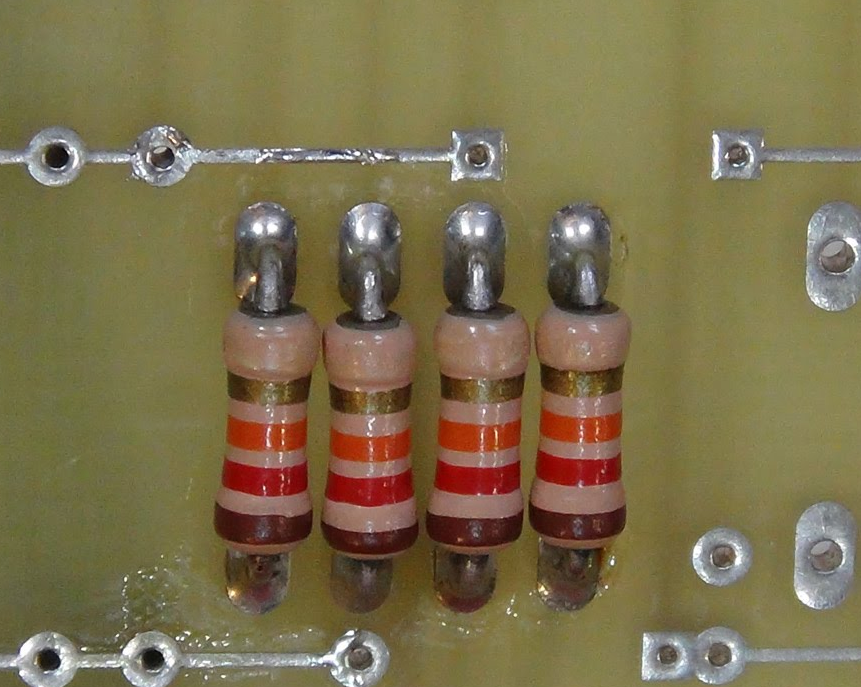
\includegraphics[width=.8\linewidth]{images/ausgangslage.png}
    \caption{M\"ogliches Bild, welches bearbeitet werden muss}
    \label{fig:ausgangslage}
\end{figure}

\newpage
\section{Welches Resultat soll ihr Algorithmus liefern?}

Die   Widerstandswerte   werden  erkannt  und  im  Bild  annotiert.  Abbildung
\ref{fig:resultat} zeigt ein m\"ogliches Resultatbild.

\begin{figure}[H]
    \centering
    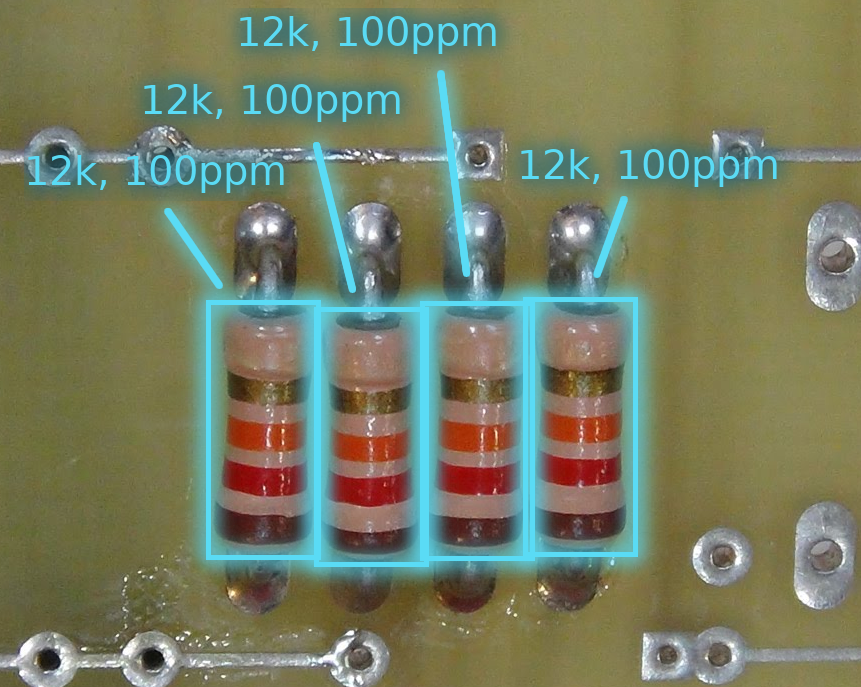
\includegraphics[width=.8\linewidth]{images/resultat.png}
    \caption{M\"ogliches Bild, welches bearbeitet wurde.}
    \label{fig:resultat}
\end{figure}


\section{Woher kommen die Ausgangsbilder?}

Von einer Digital-Kamera.

\end{document}
